\chapter{Instanciación del framework: Caso de uso}

En esta sección se presenta un caso de uso del framework Samplers tomando como ejemplo una app de ciencia ciudadana que ya se encuentra en funcionamiento, que es AppEAR, y se generará una versión usando Samplers, haciendo una breve comparación entre ambas.

\section{AppEAR}
AppEAR un sistema de ciencia ciudadana para cuidar y aprender de los ambientes acuáticos en Argentina, realizado por Joaquín Cochero, investigador del CONICET en el Instituto Platense de Limnología. Los científicos ciudadanos interactúan y colaboran en el proyecto de varias maneras, mientras que aprenden sobre los ambientes y responden a objetivos científicos. El objetivo final de AppEAR es tener un relevamiento completo y detallado de las aguas continentales de todo el territorio nacional para conocer los lugares en riesgo en los que urge trabajar. 

Los voluntarios de este proyecto descargan una aplicación para su dispositivo móvil y toman muestras para el proyecto. La aplicación guía a los usuarios a través de los pasos necesarios para tomar una muestra.\cite{appEar}

\begin{figure}[H]
  \centering
   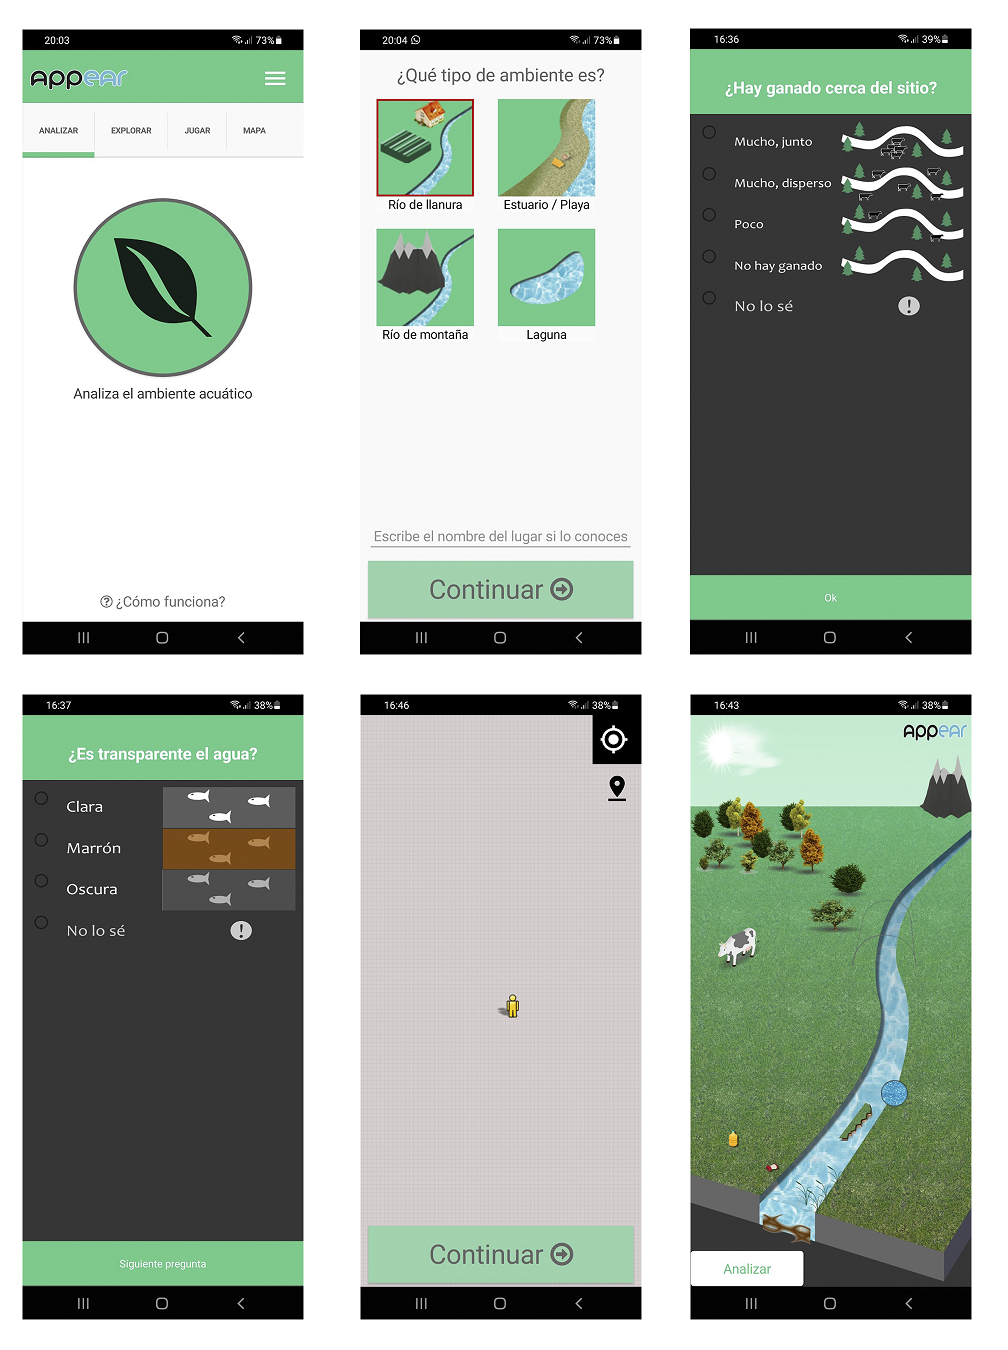
\includegraphics[scale=0.5]{06-caso_de_uso/capturas_appear.png} 
    \caption{Capturas de pantalla de la app AppEAR}
\end{figure}

Como se mencionó antes, la app va guiando a los científicos ciudadanos a través de los pasos necesarios para tomar una muestra, que son básicamente preguntas acerca del lugar que están relevando y de las cosas que ven alrededor. AppEAR diferencia 4 tipos de ambientes, que son río de llanura, río de montaña, estuario/playa y laguna, y en base a eso realiza algunas preguntas que son específicas de cada tipo y el resto preguntas comunes a los 4 tipos de ambientes. A medida que se van completando las preguntas, la app va armando una especie de dibujo del lugar con figuras que representan los elementos observados por el científico ciudadano.

Analizando todos los pasos propuestos por AppEAR se puede deducir el Workflow para tomar la muestra representado en el siguiente grafo direccional:

\begin{figure}[H] \label{img_grafo_appear}
  \centering
   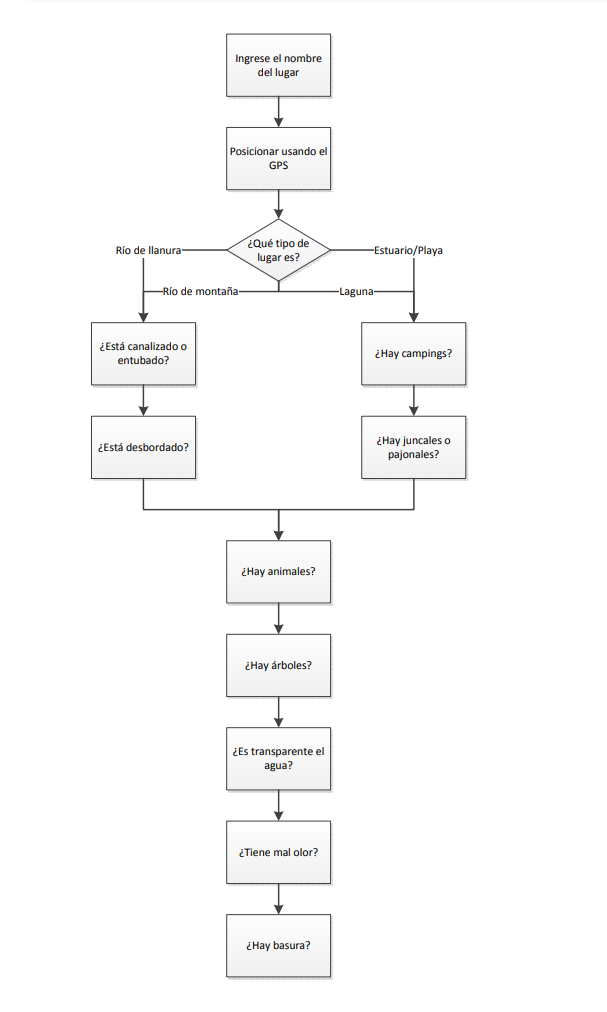
\includegraphics[scale=0.65]{06-caso_de_uso/flujo_appear.png} 
    \caption{Grafo direccional que representa el Workflow de AppEAR}
\end{figure}

\section{AppEar usando Samplers}
A continuación se muestra como sería AppEAR usando Samplers.

Observando el Workflow planteado en la figura \ref{img_grafo_appear}, se genera el archivo de configuración para Samplers de la siguiente manera:

\begin{figure}[H]\label{img_archivo_configuracion_appear}
  \centering
   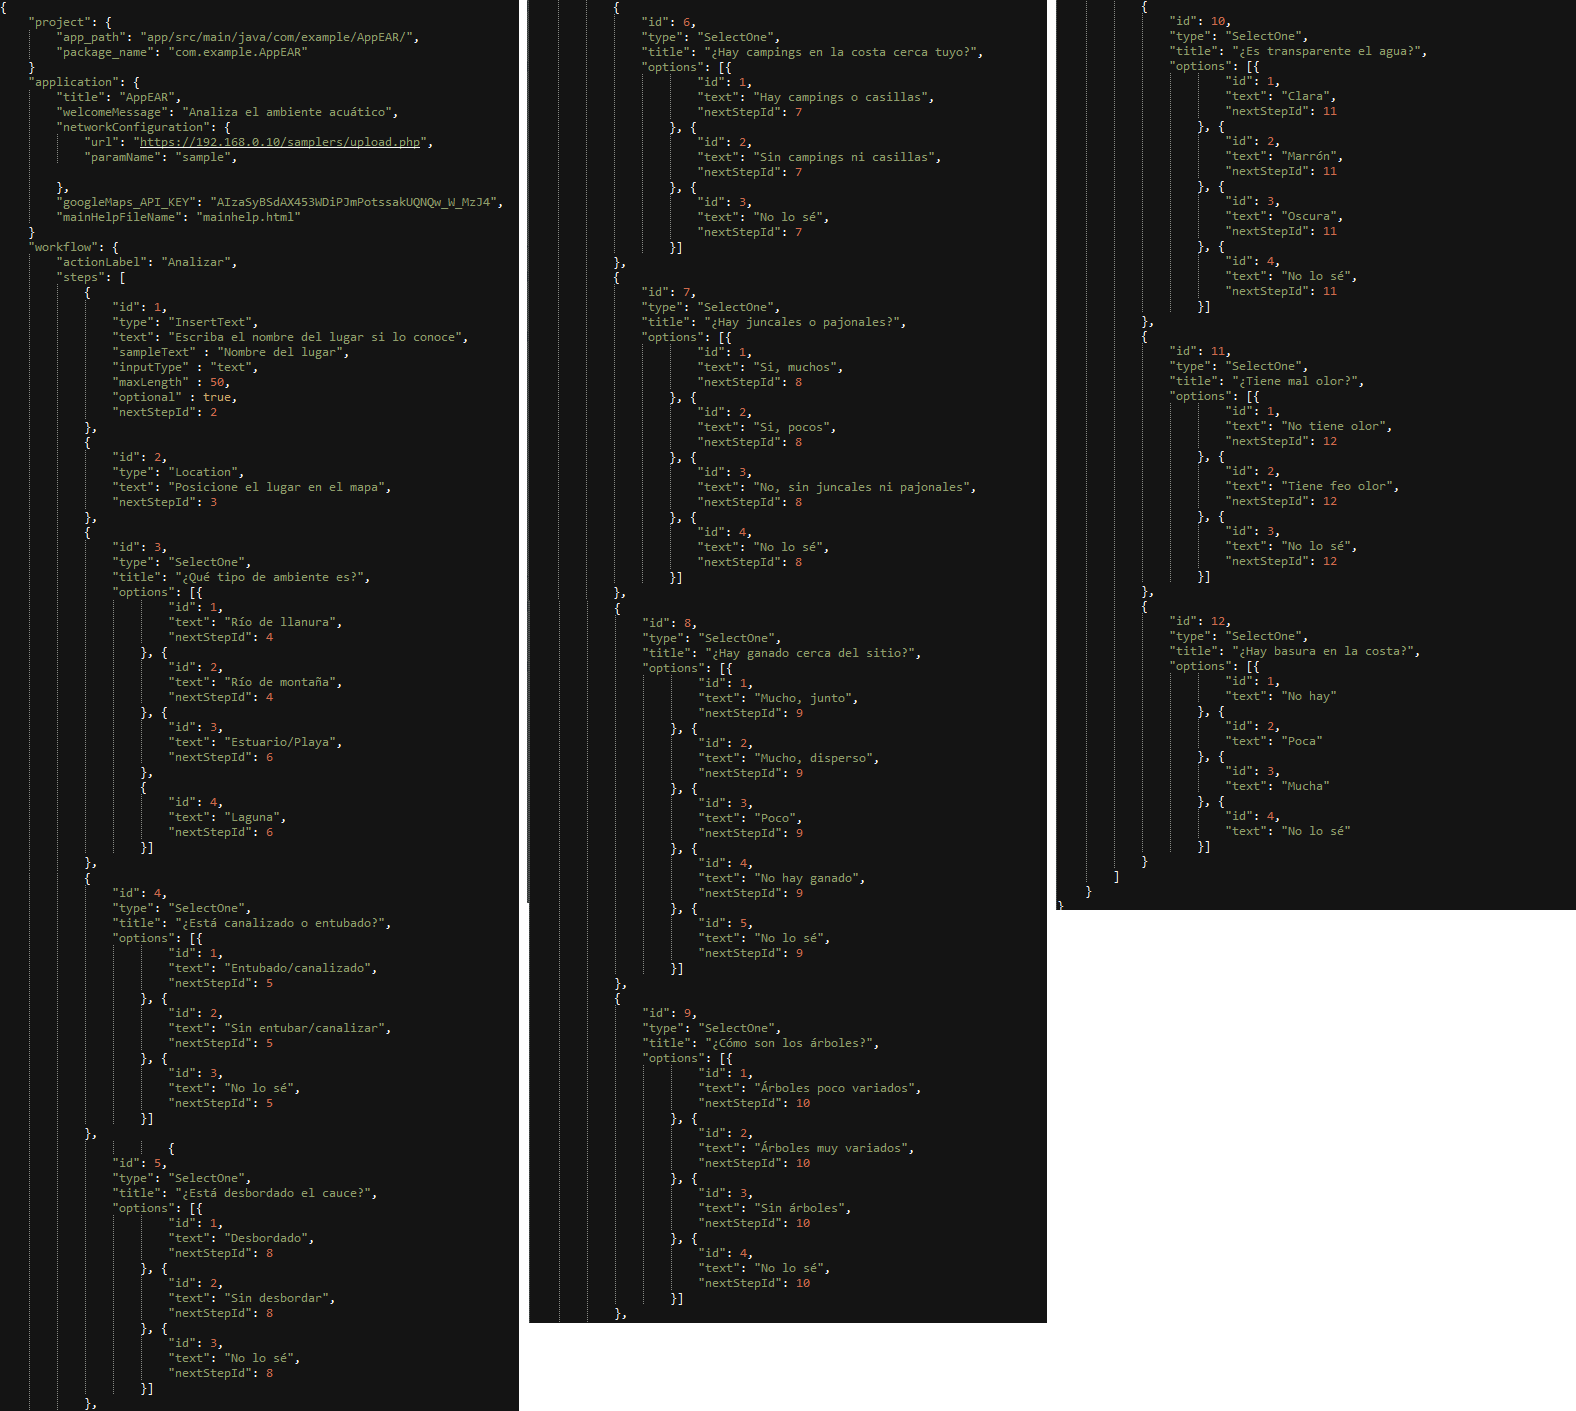
\includegraphics[scale=0.3]{06-caso_de_uso/archivo_configuracion.png} 
    \caption{Archivo de configuración para Samplers para generar una app equivalente a AppEAR}
\end{figure}

Una vez completado el archivo de configuración, se ejecuta Samplers y se genera la app.

\begin{figure}[H]
  \centering
   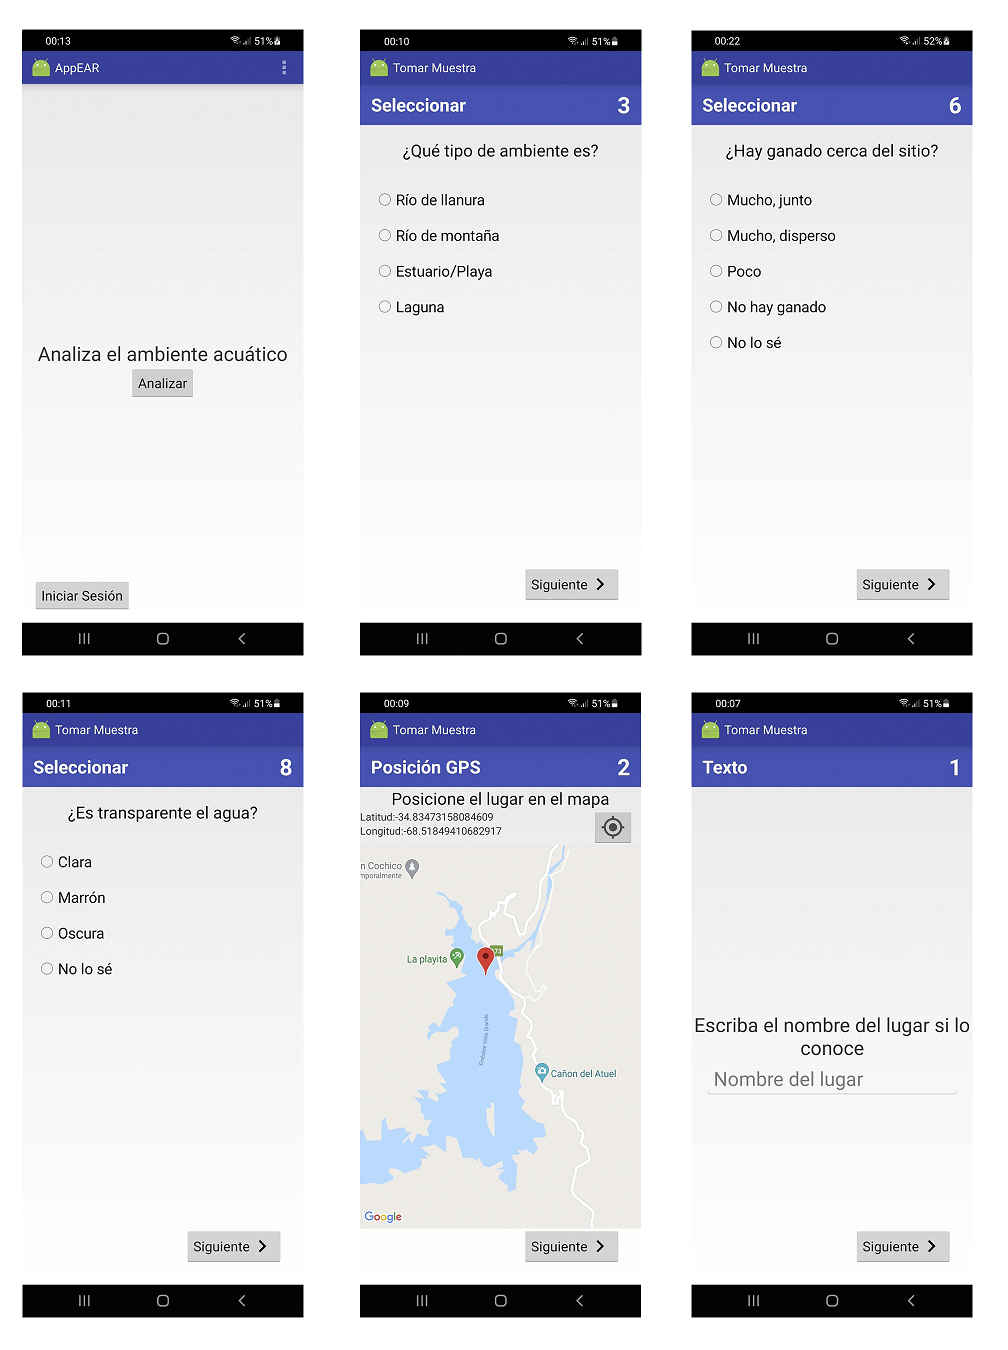
\includegraphics[scale=0.5]{06-caso_de_uso/capturas_appear_samplers.png} 
    \caption{Capturas de pantalla de la app AppEAR generada por Samplers}
\end{figure}

\section{Comparación y conclusión}
Analizando y comparando ambas aplicaciones móviles, podemos ver algunas diferencias que se detallan a continuación.


\textbf{Algunos pasos deben dividirse en dos pantallas:} por ejemplo, el paso de seleccionar el tipo de ambiente e introducir el nombre del lugar están en una misma pantalla en AppEAR, pero en la app generada por Samplers están en dos pantallas diferentes, ya que se resuelven con un SelectOneStep para la selección del tipo de ambiente y un InsertTextStep para introducir el nombre del lugar.

\begin{figure}[H]
  \centering
   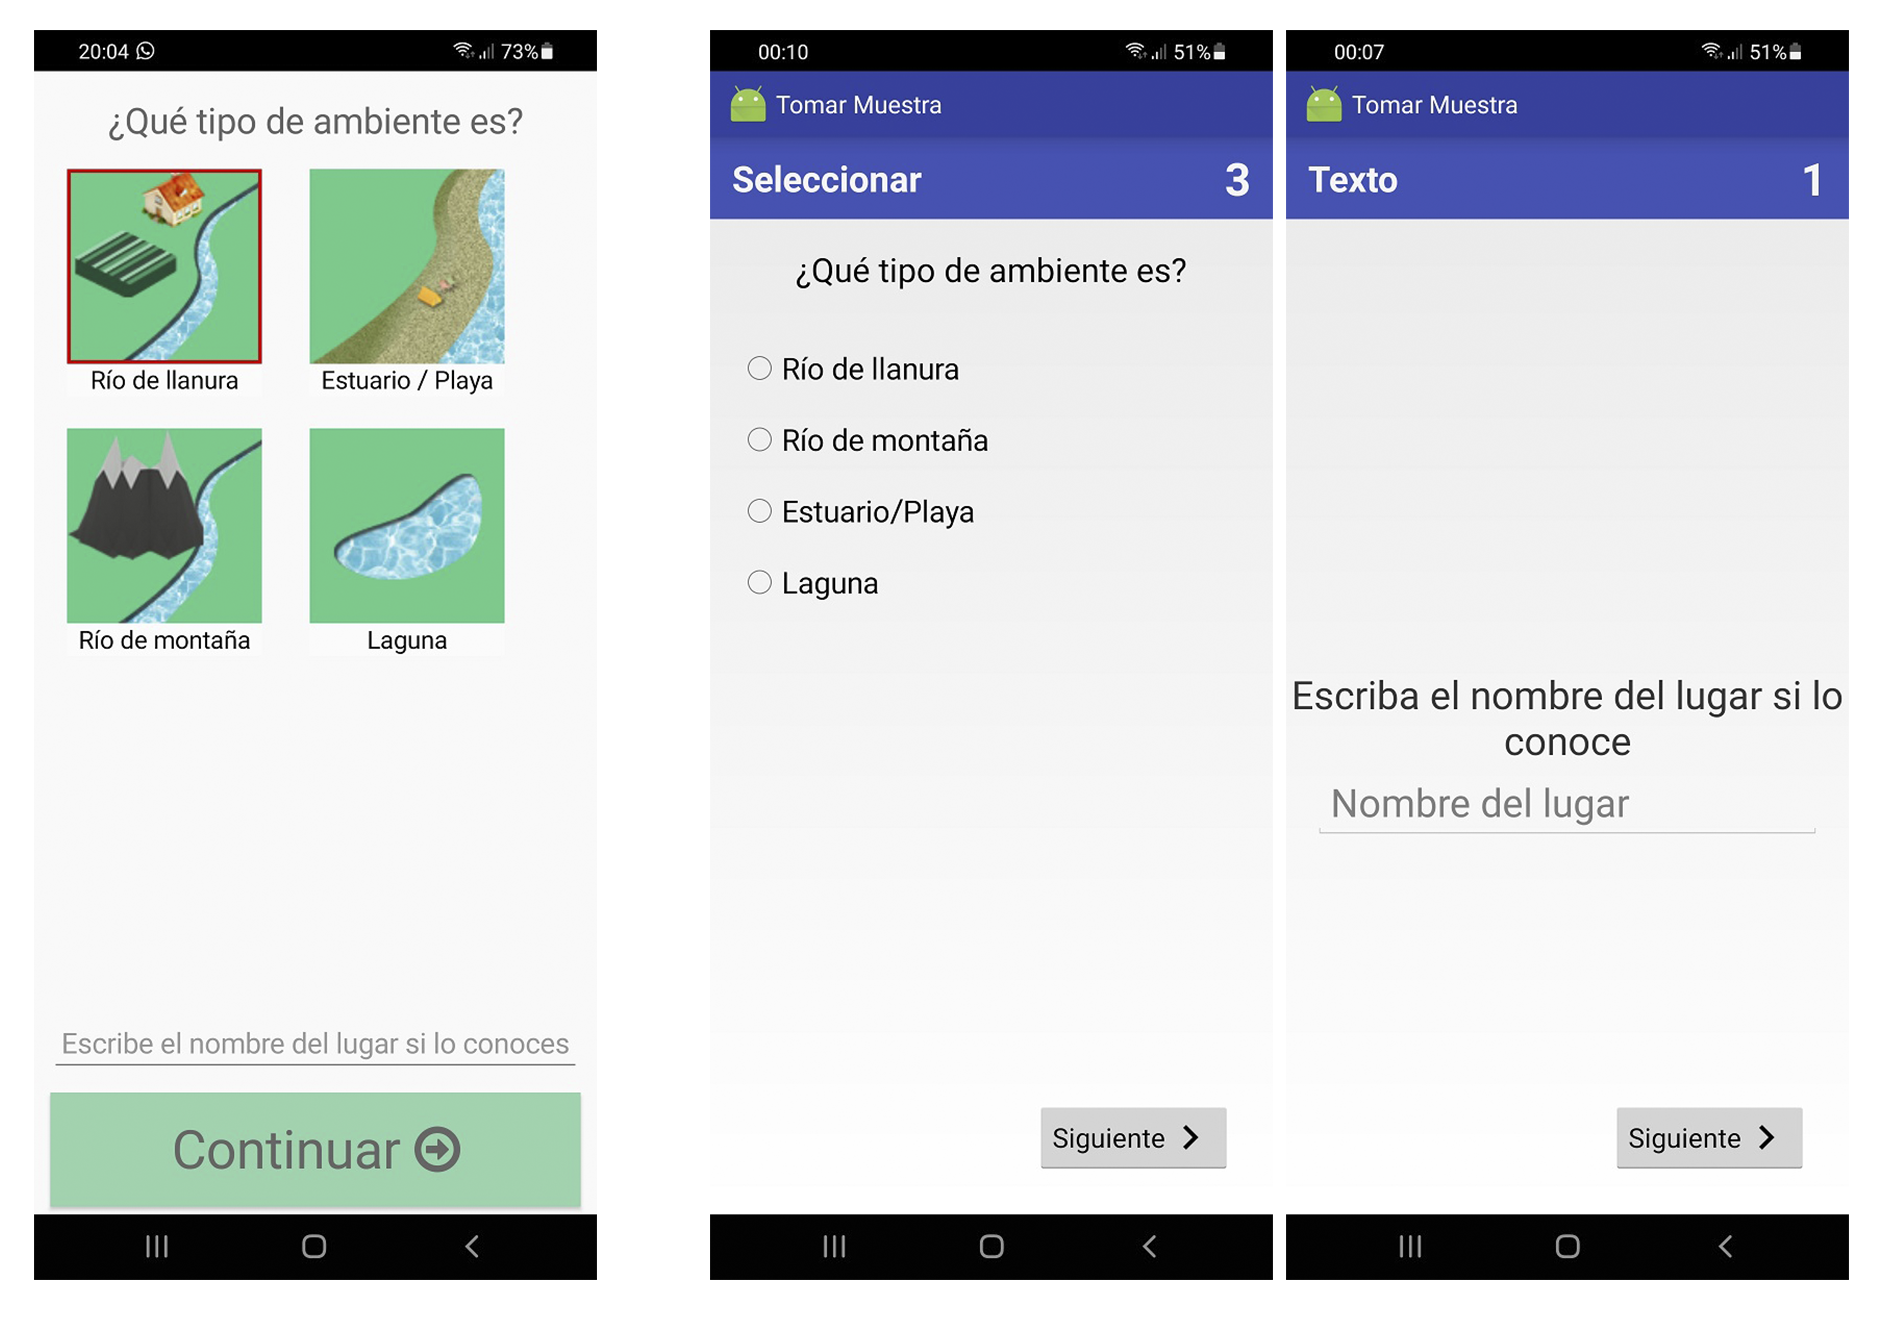
\includegraphics[scale=0.8]{06-caso_de_uso/tipo_y_nombre.png} 
    \caption{Izquierda: tipo de ambiente y nombre en una sola pantalla (AppEAR). Derecha:  tipo de ambiente y nombre en dos pantallas (Samplers)}
\end{figure}

\newpage

\textbf{La selección de opciones no tiene imágenes:} en la mayoria de los pasos de seleccionar alguna opción en AppEAR tienen imágenes de referencia al lado de cada opción, pero en la app generada por Samplers estas imágenes no están disponibles porque SelectOneStep solo muestra los radio-buttons con el texto de la opción para seleccionar.

\begin{figure}[H]
  \centering
   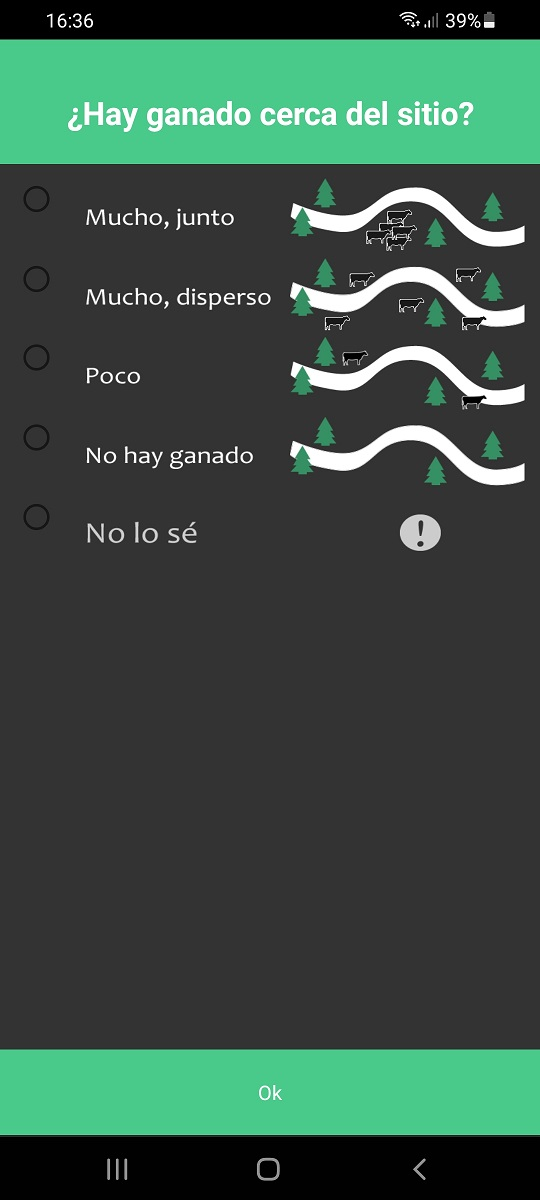
\includegraphics[scale=0.3]{06-caso_de_uso/appear_ganado.jpg} 
   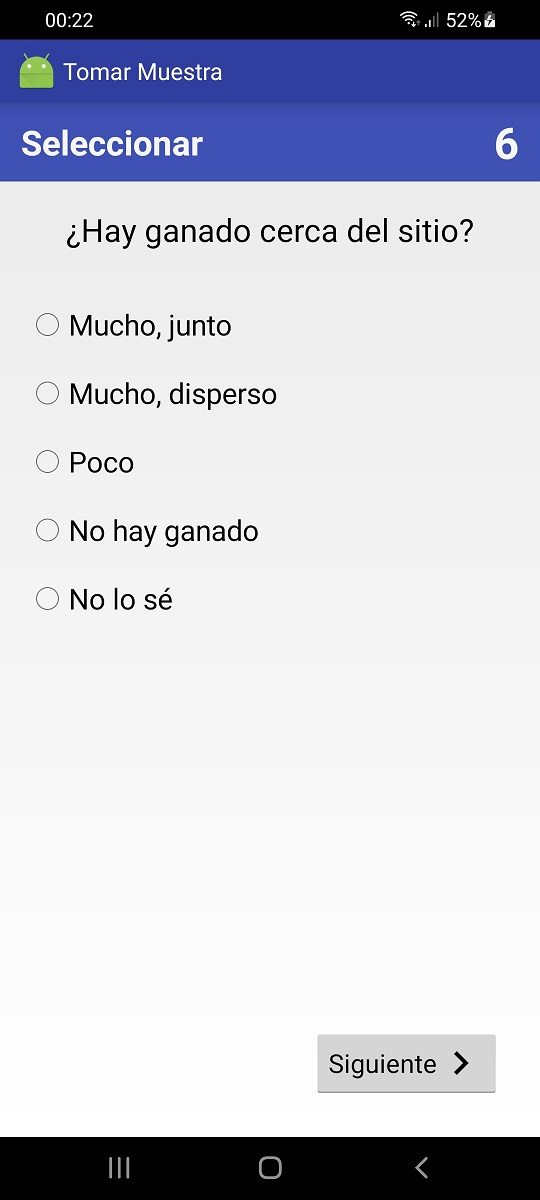
\includegraphics[scale=0.3]{06-caso_de_uso/samplers_ganado.jpg} 
    \caption{Izquierda: selección con imágenes (AppEAR). Derecha:  selección simple (Samplers)}
\end{figure}

\newpage

\textbf{Pantalla principal sin imágenes:} la pantalla principal en AppEAR tiene una imagen de fondo, que no está en la app generada por Samplers. Igualmente esta imagen se puede agregar con bastante facilidad, ya que como Samplers genera el código de la app la Activity principal (que es la que provee la pantalla principal) se puede editar, y Android Studio provee herramientas visuales muy intuitivas para diseñar la interfaz de una pantalla.

\begin{figure}[H]
  \centering
   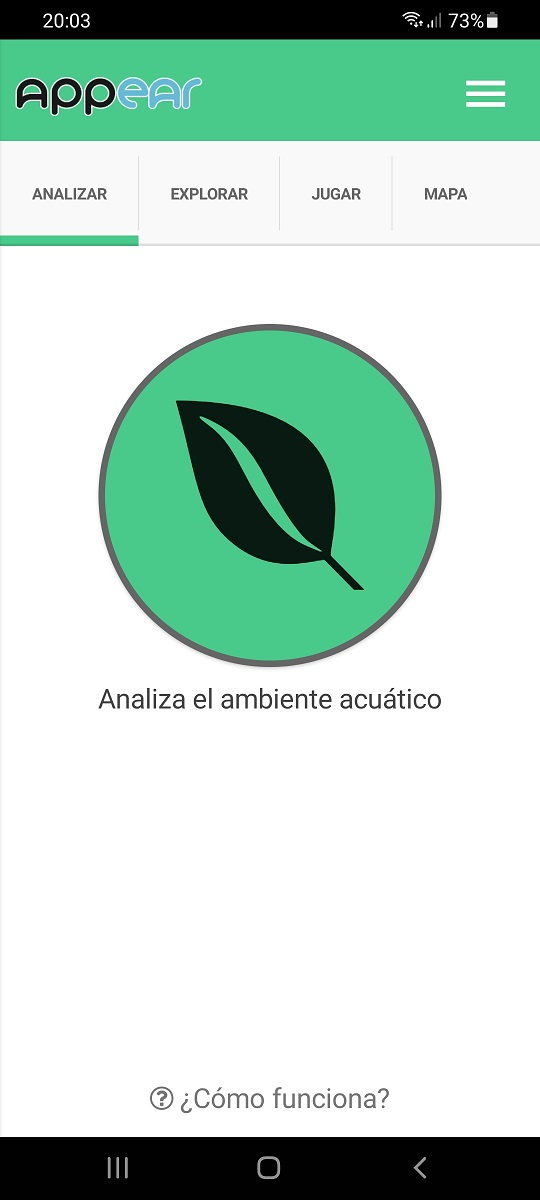
\includegraphics[scale=0.3]{06-caso_de_uso/appear_main.jpg} 
   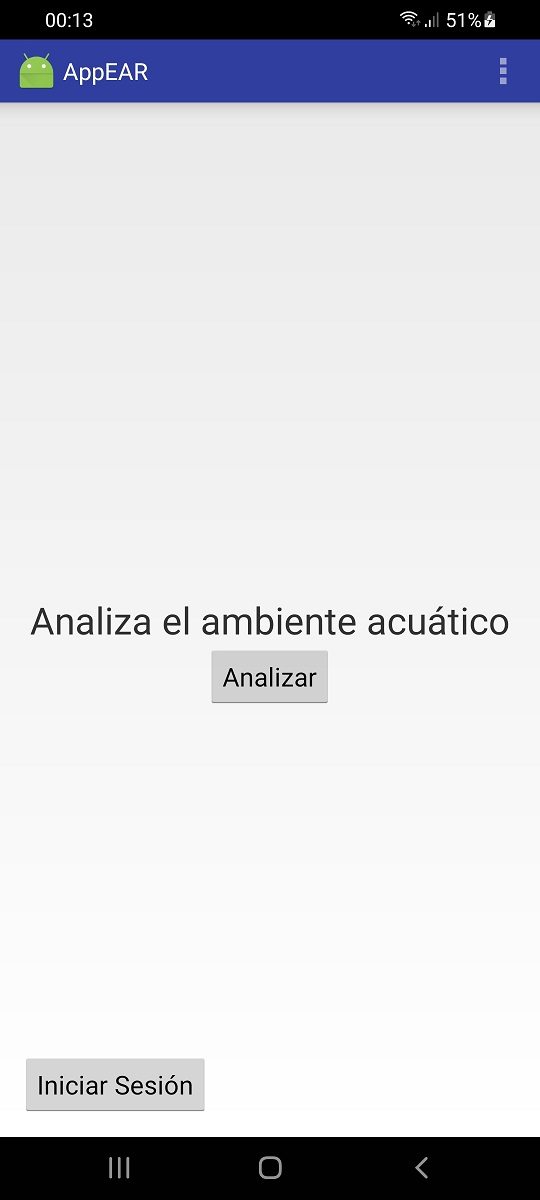
\includegraphics[scale=0.3]{06-caso_de_uso/samplers_main.jpg} 
    \caption{Izquierda: pantalla principal con imágenes (AppEAR). Derecha:  pantalla principal sin imágenes (Samplers)}
\end{figure}

\newpage

\textbf{Pantallas especiales que no están:} hay pantallas especiales en AppEAR que no representan ningún paso para tomar la muestra, pero que están dentro de la secuencia, como por ejemplo la pantalla que va mostrando un esquema del lugar que se está analizando con imágenes predeterminadas a medida que el usuario va completando los pasos. En Samplers no hay un Step que pueda representar eso, por lo que no se pueden agregar.

\begin{figure}[H]
  \centering
   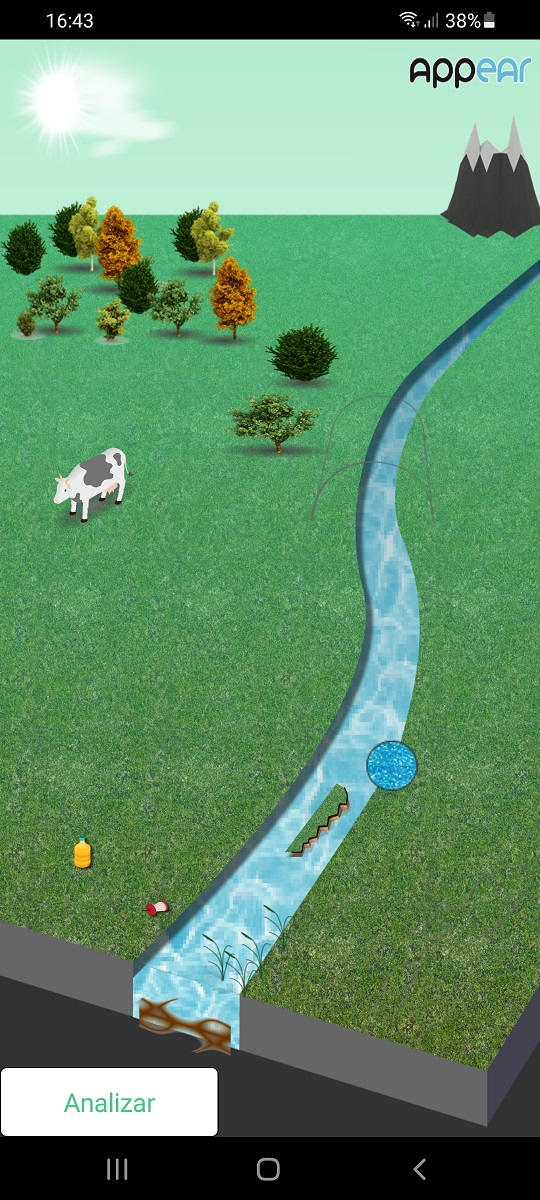
\includegraphics[scale=0.3]{06-caso_de_uso/appear_esquema.jpg} 
    \caption{Ejemplo de pantalla especial (AppEAR)}
\end{figure}

\newpage

\textbf{Los mapas se muestran correctamente:} en AppEAR al posicionar el lugar que se está analizando, si bien toma la posición con el GPS correctamente, el mapa de fondo no se muestra. En Samplers se muestra el mapa que provee la API de GoogleMaps y que funciona correctamente en todos los dispositivos móviles con Android.

\begin{figure}[H]
  \centering
   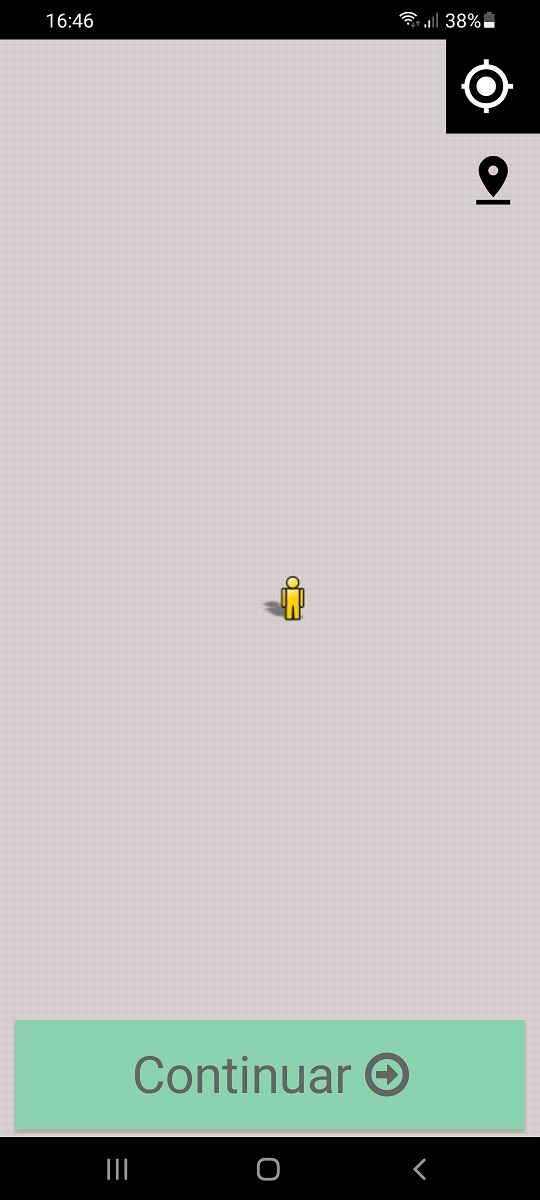
\includegraphics[scale=0.3]{06-caso_de_uso/appear_mapa.jpg} 
   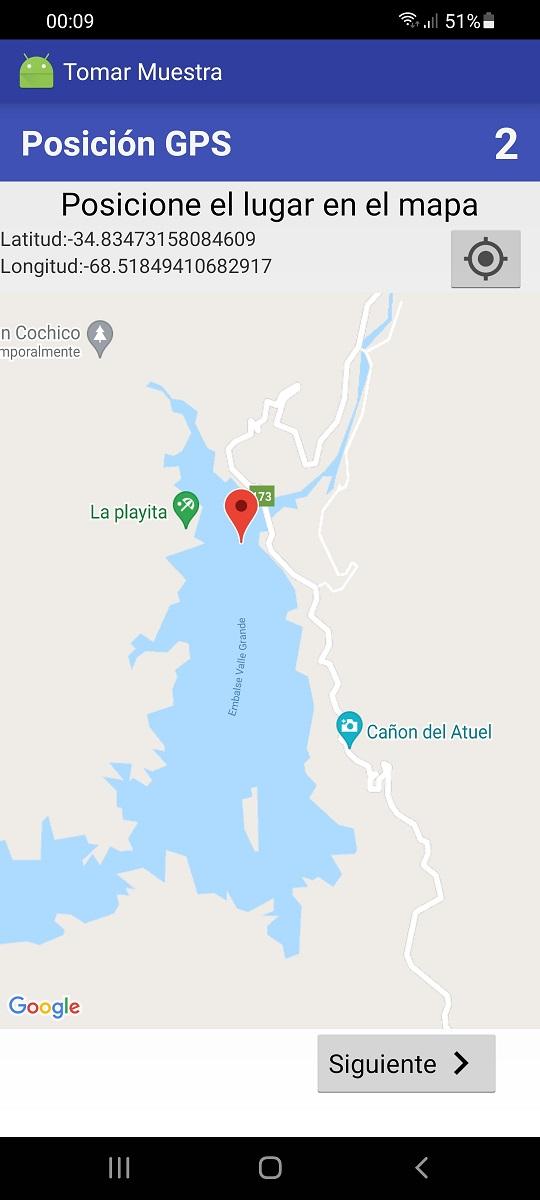
\includegraphics[scale=0.3]{06-caso_de_uso/samplers_mapa.jpg} 
    \caption{Izquierda: mapa con problemas de visualización (AppEAR). Derecha:  mapa que se muestra correctamente (Samplers)}
\end{figure}

Más allá de las diferencias encontradas, la app generada por Samplers es funcionalmente equivalente a AppEAR y sirve para recolectar las muestras que necesita el proyecto. La ventaja principal de Samplers es que no se requieren conocimientos de programación para generar la app, sólo hay que completar el archivo JSON que se muestra en la figura \ref{img_archivo_configuracion_appear}, lo que también reduce considerablemente el tiempo de desarrollo de la app. Además como Samplers genera el código de la app, la misma se puede editar para personalizarla y agregarle más funcionalidades, por lo que puede ser usada por un programador como punto de partida de un proyecto.

